%! Author = louis
%! Date = 28-10-22

% Preamble
\documentclass[12pt, a4paper, oneside]{article}

% Packages
\usepackage[french]{babel}
\usepackage[margin=2.5cm]{geometry}
\usepackage[utf8]{inputenc}
\usepackage{graphicx}
\usepackage[colorlinks=true, pdfborder {0 0 0},linkcolor=black]{hyperref}
\usepackage{listings}
\usepackage{color}
\usepackage{lipsum}
\usepackage[nomain, toc, xindy, acronym]{glossaries}
\usepackage{wrapfig}
\usepackage{fancyhdr}
\usepackage[T1]{fontenc}
\usepackage[labelformat=empty]{caption}
\usepackage{titlepic}
\usepackage[xindy]{imakeidx}
\usepackage[backend=bibtex]{biblatex}
\usepackage{pdfpages}
\hypersetup{
    colorlinks=true,
    linkcolor=black,
    filecolor=magenta,
    urlcolor=cyan,
    pdftitle={Clever-Party-Thrower, une application web hébergée via Kubernetes et Ansible},
    pdfpagemode=FullScreen,
}
\fancyhf{}
\fancyhead[LO,RE]{\sffamily\itshape \leftmark}
\fancyfoot[C]{\thepage}
\pagestyle{fancy}

\makeatletter
\renewcommand\paragraph{\@startsection{paragraph}{4}{\z@}%
% display heading, like subsubsection
{-3.25ex\@plus -1ex \@minus -.2ex}%
{1.5ex \@plus .2ex}%
{\normalfont\normalsize\bfseries}}
\setcounter{secnumdepth}{4}
\makeatother
% Document
\begin{document}
    \begin{titlepage}
        \begin{center}
            \vspace*{1cm}

            \Huge
            \textbf{Clever-Party-Thrower, une application web hébergée via Kubernetes et Ansible}

            \vspace{0.5cm}

            \vspace{1.5cm}

            \textbf{Louis De Wilde}

            \vfill

            
\includegraphics[width=0.65\textwidth]{images/EPHEC_logo.svg}
            \vfill
            \vspace{0.8cm}
            \Large
            Technologie de l'informatique 3TL2 \\
            Ephec : Av. du Ciseau 15, 1348 Ottignies-Louvain-la-Neuve\\
            Novembre 2022

        \end{center}
    \end{titlepage}
    \thispagestyle{empty}
    \newpage
    \setcounter{page}{0}
    \begin{KeepFromToc}
        \tableofcontents
    \end{KeepFromToc}
    \newpage
    % \bibliography{main}
    %\bibliographystyle{plain}


    \section{Introduction}\label{sec:introduction}
    

Dans le monde d'aujourd'hui, les étudiants et les personnes en général sont souvent amenés à organiser des événements, tels que des soirées ou des fêtes entre amis.
Cependant, gérer les aspects logistiques de ces événements peut s'avérer compliqué, notamment lorsqu'il s'agit de fixer une date, de répartir les coûts et de coordonner les participants.
Afin de faciliter ce processus et d'améliorer l'expérience de l'organisation de fêtes, j'ai décidé de développer une application web nommée "Clever Party Thrower".
Cette application permettra aux utilisateurs de gérer efficacement tous les aspects importants de l'organisation d'un événement,
y compris les dépenses, les courses voir meme la musique, les covoiturages et bien plus encore.\\\\

Dans ce rapport, je présenterai les différentes étapes du développement de l'application Clever Party Thrower,
en commençant par le choix du sujet et en détaillant le cahier des charges, l'analyse de la problématique, la conception et la réalisation du projet.
J'aborderai également les aspects liés à la sécurité, la gestion des versions, les tests et la documentation du code.\\
Un accent particulier sera mis sur l'adoption de pratiques de développement modernes, telles que l'intégration continue (CI) et le déploiement continu (CD), afin d'assurer la qualité et la fiabilité du code tout au long du cycle de développement.
De plus, je discuterai des choix d'hébergement pour l'application, en explorant les options d'auto-hébergement voir meme compatible avec le cloud.\\

Enfin, je terminerai en présentant une conclusion sur le travail accompli, les défis rencontrés et les perspectives d'amélioration pour le futur.
    \newpage


    \section{Choix du sujet}\label{subsec:choix-du-sujet}
    Dans le contexte actuel, les étudiants et les personnes qui aiment s'amuser en général organisent souvent des soirées ou des fêtes entre amis.
Pourtant, planifier et organiser de tels événements peut s'avérer difficile, en particulier lorsqu'il s'agit de fixer une date convenant à la majorité des participants et de gérer les dépenses.
Les défis augmentent lorsque le nombre de participants s'accroît.\\

Afin de résoudre ce problème, j'ai décidé de créer une application web qui facilite l'organisation de petites fêtes estudiantines.
Ce sujet présente un intérêt technique, car il implique la création d'une plateforme en ligne accessible à un large public.
De plus, il répond à un besoin réel des utilisateurs qui cherchent à simplifier l'organisation de leurs événements et à réduire les efforts nécessaires pour coordonner les participants.\\

L'application apportera une plus-value en proposant des fonctionnalités spécifiques pour gérer les aspects clés de l'organisation d'une fête, telles que la répartition des coûts,
la gestion des courses et le choix d'une date.
En outre, elle offrira un positionnement unique par rapport aux solutions existantes en offrant toutes ces fonctionnalités au sein d'une meme application.\\

Enfin, le sujet a été validé par un cours sondage au pres d'une vingtaine d'étudiants et une recherche d'application similaire deja existante, qui ont montré un intérêt pour une telle solution.
Ce travail représentera une charge de travail suffisante, estimée à environ 350 heures.
    \newpage


    \section{Cahier des charges}\label{sec:cahier-des-charges}
    \subsection{Contexte}\label{subsec:contexte}
Dans le contexte des étudiants et des personnes qui aiment s'amuser, l'organisation de petites fêtes estudiantines est souvent une tâche complexe.
Il est nécessaire de prendre en compte la date, les dépenses, la logistique et les préférences des participants.
Pour faciliter ce processus, une application web est proposée pour assister les organisateurs et les participants dans la gestion des différents aspects de l'événement.

\subsection{Besoin du client}\label{subsec:besoin-du-client}
\begin{itemize}
    \item Permet de répartir équitablement les frais engendrés par la fête
    \item Crée une liste des courses pour la soirée (éventuellement une répartition si toutes les courses ne se font pas au meme endroit ?)
    \item Connaître qui a amène quoi à la fête
    \item Crée différents évènements
    \item Est accessible grâce à un simple lien
    \item Est pourvu d'un système de connexion et de création de compte simple
    \item Permet de trouver une date d’évènement qui convient au plus grand nombre de participants
\end{itemize}

\subsection{Fonctionnalités optionnelles}\label{subsec:fonctionnalites-optionnelles}
\begin{itemize}
    \item Permet de créer une playlist commune (sur laquelle chacun a la possibilité d'ajouter des titres)
    \item Permet au conducteur de connaitre son trajet de covoiturage
    \item Permet au participant d'organiser facilement des covoiturages
    \item Calcule et reparti automatiquement les frais de transport entre les différents covoitureurs
\end{itemize}

\subsection{Contraintes}\label{subsec:contraintes}
\begin{itemize}
    \item Accessible sur toutes les plateformes (Android, IOS, Mac, Windows, Linux)
    \item Le système de création de compte doit être simple
    \item Les données des utilisateurs seront sécurisées
    \item L’application doit être auto-hébergable
    \item Respect des réglementations en matière de protection des données (GDPR)
\end{itemize}

\subsection{Méthodologie}\label{subsec:methodologie}
Pour la réalisation du projet, une méthodologie inspirée de Scrum sera utilisée, avec la division des demandes de l'utilisateur en petites tâches.
L'outil FocalBoard sera utilisé pour organiser et suivre l'avancement des tâches.
Le code sera géré sur GitHub, avec l'intention d'utiliser l'intégration et le déploiement continus, ainsi que des tests automatisés pour certaines parties du projet.
L'étudiant travaillera en étroite collaboration avec le rapporteur pour valider les différentes étapes du projet et s'assurer que les attentes sont respectées.

\subsection{Interactions avec le client (et/ou le rapporteur)}\label{subsec:interactions-avec-le-client-(et/ou-le-rapporteur)}
L'étudiant fournira des mises à jour régulières au rapporteur sur l'avancement du projet, et sollicitera des conseils et des orientations si nécessaire.
Des réunions périodiques pourront être organisées pour discuter des problèmes, des progrès et des améliorations possibles.
    \newpage


    \section{Analyse}\label{sec:analyse}
    %! Author = louis
%! Date = 28-10-22

Le projet ayant comme contrainte principale d'etre disponible sur toute les platformes majeur une base web me parait évident.
Pourtant, le web vient aussi avec la limitation pricipale qu'est le besoin de connection permanente au serveur,
pour remedier a ce probleme un PWA ( Application Web Progressive ) nous permetrais de beneficiez des avantages du web,
tout en permetant aux utilisateurs de concerver une version locale de l'application.
De plus une PWA permet d'etre instalée comme une application native Android ou IOS pour les platformes mobiles ce qui facilite l'accès.\\\\

Une PWA comme toute application web necesite plusieurs composant:
\begin{itemize}
    \item Un back-end
    \item une Base de Donnée
    \item une Interface definie pour le back-end ( API )
    \item un front-end
\end{itemize}
\subsubsection{TypeScript}
Pour ce projet j'ai decidé d'utiliser le meme language pour les 2 composant majeurs que sont le front et le back end.
Plusieurs choix s'offrais alors a moi , JavaScript, Kotlin, TypeScript ou n'importe quel language compilable en web assembly\\
JavaScript n'etait pas vraiment un bon choix vu qu'il ne propose pas de typage ce qui rend le code moin predictible et robuste.
Kotlin est un bon candidat il offre un typage statique mais propose de l'inference de type, peu etre transpiler vers du JavaScript ou du web assembly,
les outils de developement pour kotlin sont aussi tres bon mais la documentation pour une utilisation web est plutot pauvre comparer aux autres options.\\
TypeScript a quand a lui tout les avantage de Kotlin, grace au typage fort, et profite aussi de la documentation et des outil javaScript grave a ca nature de superset.
Lorsque l'on develope un produit web surtout pour un developeur Full Stack TypeScript est l'idéal.
Ces outils, l'enviromement JavaScript, la securité des Types et du null, la documentation.
Pour tout ces raison TypeScript est le language idéal pour le developement Web.
\subsection{Back-end}\label{subsec:back-end}
Le serveur back-end doit etre capable de mettre à disposition les données nécessaire au fonctionnement de l'application.
Cependant, le back-end sera aussi responcable des calculs d'équilibrage des dépenses, des matching de covoiturage et des trajets.\\\\
Connaissant deja Express.js et Spring ( Kotlin ) je me suis naturellement tourné vers ces derniers néanmoins je désirais utiliser du TypeScript pour ce projet.
Express.js est compatible avec TypeScript mais Spring ne l'est pas, Express.js est leger, minimaliste et propose une bonne documentation,
Spring est generaliste propose des outils de generation de code et utilise une systeme d'injection de dependance.
Ce qu'il me fallait etait une hybride entre Spring et Express.js.
Apres quelque recherche, j'ai trouvé un framework appler Nest.js, ce dernier supporte nativement TypeScript, propose une documentation ecxelante,
propose un CLI permetant de generer du code boiler-plate, reste simple et leger, Utilise de l'injection de dependance et est tres utiliser et apprecier par d'autre developeurs.
J'ai donc decider d'utiliser Nest.Js pour ce projet.

\subsubsection{ORM}
Nest.Js ( que je vais appeller Nest à partir de maintenant ) n'est pas un framework batteries included comme le son Spring ou Laravel,
Il m'a alors fallu choisir aussi un ORM pour interfacer avec ma base de donnée.
Dans la Documentation de Nest, il y a des exemples de configuration avec les ORM les plus Utiliser avec Nest et TypeScrip.
Ces derniers sont Sequelize, TypeOrm et Prisma,
ayant eu une experience avec Sequelize plus tot mauvaise lors de mon projet de dev3, j'ai decider de regarder du côté de prisma.
Prisma est une ORM un peu particulière dans le sens ou il propose d'utiliser une schema prisma pour definir ces entités plutôt que le code TypeScript.
Cella me paraissait une tres bonne chose vu que prisma generais alors lui meme les differents DTO nécessaire.
Il c'est cependant averer que a l'utilisation prisma n'est pas l'ideale surtout lorsque l'on désire le coupler à une API graphQl
À cause de son schema particulier, je devais definir le forma de mes entitée à 2 endroits et tout de meme crée manuelement mes DTO.
J'ai donc decider de jeter une oeuil à TypeOrm, celui-ci propose de definir les entités via des annotations TypeScript.
Ce qui me permet d'utiliser une seule classe pour definir mon entitée d'orm et de graphQl de plus TypeOrm est mieux
documenter grace au support d'une comunauter plus large.


\subsection{La base de donnée}\label{subsec:la-base-de-donnee}
Ma base de donnée devais me permetre 2 chose, stocker des données geographique et faire des operation sur ces données.
Le seul choix qui s'offrait à moi compatible avec TypeOrm etait postgress avec une extention nomer POSTGIS .
Postgres est une base de donnée tres utiliser en production et est tres performante et stable.

\subsubsection{Structure de donnée}
Pour stoquer tout les donnée nescesaire au fonctionement de l'application il nous faut une structure de donnée coherante.
Voici un shema de la base de donnée et de ca structure:
%Todo: Shema DB


\subsection{L'API back end}\label{subsec:l'api-back-end}
Il existe plusieurs types d'API tres utiliser pour le Back-end mais les plus populaires sont le REST et le SOAP.
SOAP est de moin en moin utiliser dû à la complexité intrinsec du xml et à sa lourdeur.
Il nous reste donc REST qui est une bonne solution, mais nescecite pour presque chaque requete de recuperer des données qui ne seront pas toujour consomée par le client
Avec Rest l'on récupère une entitée complete tous les champs sont renvoyés.
C'est pour cela que graphQl a ete crée, non seulement graphQL utilise un typage fort via un schema defini et exposer par le serveur,
mais en plus graphql permet de ne recuperer que les champs nescesaire au client grace au GQL .




\subsection{Front-end}\label{subsec:front-end}
Pour ce qui est de l'interface utilisateur ( le front end ) j'ai decidé d'utiliser angular car ce framework utilise TypeScript nativement et supporte aussi les PWA
TypeScript est important, parce qu'il permet d'éliminer les bugs lier au typage d'objet avant meme l'execution du programe.
Angular etant un framework orienter m'oblige aussi à suivre une architecture propre qui permet de rendre independant les differents composants du projet.

    \newpage


    \section{Hebergement et aspects reseaux}\label{sec:hebergement-et-aspects-reseaux}
    Afin d'héberger Clever Party Thrower, plusieurs possibilités s'offrent au client.
Celles-ci dépendent de son budget, de l'infrastructure dont il dispose et du nombre d'utilisateurs qui devront être servis.

\subsection{docker-compose}\label{subsec:docker-compose}
L'application, étant packagée dans des conteneurs Docker, peut être déployée très facilement dans un environnement restreint grâce à Docker et Docker Compose.
Durant le développement de l'application, j'ai souhaité permettre à des utilisateurs potentiels du service de tester certaines parties de l'interface.\\

J'ai donc décidé d'héberger un stack Docker Compose sur un petit serveur de mon homelab.
Le stack que j'ai choisi de décrire dans la documentation est minimaliste, il comprend le strict nécessaire pour héberger et utiliser l'application.
Le fichier docker-compose comprend le backend, la base de données et le frontend hébergé par un serveur nginx.

\subsection{kubernetes}\label{subsec:kubernetes}
Lorsque le client dispose d'une infrastructure performante, il a la possibilité de déployer l'application sur un ou plusieurs clusters Kubernetes.
Durant le développement de l'application, je me suis intéressé à l'orchestration de conteneurs avec Kubernetes,
ce qui m'a conduit à proposer des fichiers de configuration pour héberger le site web et son serveur.\\

En parallèle de ma formation sur Kubernetes, j'ai également exploré Ansible et ai adapté un projet open-source existant afin de permettre le déploiement de Clever Party Thrower sur un cluster Kubernetes en une seule commande.
Ce playbook Ansible facilite le déploiement d'un cluster K3S complet, avec ou sans haute disponibilité.
De plus, le playbook déploie également des applications telles que kubeVip, MetalLB, Rancher, Traefik, Cert-manager, LongHorn et ArgoCD.

\subsubsection{Le Playbook}
Le Playbook permet de déployer Kubernetes sur plusieurs machines, appelées nodes, afin d'ajouter de la résilience au cluster.
Plus il y a de nodes, plus le cluster peut en perdre sans interruption de service.
Les différentes applications utilisées pour permettre cette haute disponibilité sont les suivantes : \\

\begin{itemize}
    \item \textbf{Kubernetes} : Kubernetes synchronise et répartit toutes les configurations et les ressources entre les différentes nodes
    pour garantir que chacune d'entre elles peut à tout moment gérer le trafic.\\

    \item \textbf{Kubevip} : Kubevip sert à créer une adresse virtuelle pour la gestion du cluster.
    Cette adresse virtuelle permet de conserver une connexion avec le cluster tant qu'au moins une des nodes master est en ligne et fonctionnelle .\\

    \item \textbf{MetalLB} : MetalLB est un load balancer qui, comme son nom l'indique, permet d'équilibrer la charge de travail.
    Il attribue également des adresses IP à des pods (conteneurs dans Kubernetes) en fonction de leur nom ou espace de nom et ce, dans une plage définie .\\

    \item \textbf{Cert-manager} : Cert-manager permet de créer et renouveler les différents certificats via Let's Encrypt,
    en plus de permettre à Kubernetes de les gérer comme toute autre ressource, et donc de les synchroniser entre les différentes nodes.\\


    \item \textbf{Traefik} : Traefik sert de reverse proxy, protégeant ainsi les différents services du cluster.
    Il gère également la distribution de la charge pour les requêtes \Gls{https} .\\
    \item \textbf{Longhorn} : Longhorn permet de créer des volumes partagés et disponibles sur plusieurs nodes en même temps,
    garantissant ainsi aux pods exploitant ces volumes qu'ils seront toujours accessibles.\\
\end{itemize}

\subsection{Les Conteneurs}\label{subsec:les-conteneurs}
Le conteneur back-end est relativement simple.
Il utilise une image node:latest.
Une fois le code source transpilé, le résultat de cette compilation est copié dans l'image.\\

Le conteneur pour la base de données utilise quant à lui une simple image de PostGIS.
PostGIS est une extension de PostgreSQL qui permet la manipulation de points géographiques directement sur la base de données.\\

Le conteneur front-end est plus complexe.
Basé sur une image nginx, il intègre le résultat de la compilation Angular dans le dossier où nginx cherche les fichiers à servir.
Nginx sert donc le front end, et agit également comme un proxy pour permettre au front end d'accéder au backend.

\subsection{Mon choix}\label{subsec:mon-choix}
En tant que client, j'ai choisi d'héberger l'application via docker-compose.\\

À l'origine, mon objectif était de créer un cluster Kubernetes distribué entre plusieurs machines virtuelles pour simuler
diverses machines physiques, et de déployer l'application sur ce cluster.
Cependant, Kubernetes, et surtout la haute disponibilité, exige beaucoup de ressources, que mon serveur ne pouvait pas supporter.
Les différentes machines virtuelles manquaient constamment de mémoire ou d'espace disque.\\

J'ai ainsi décidé d'utiliser un simple docker-compose pour optimiser les ressources de mon serveur,
permettant d'héberger toutes mes applications plutôt que de se limiter à une seule avec des performances médiocres.
À l'avenir, si les limites matérielles ne sont plus un obstacle, j'envisagerai de déployer une infrastructure Kubernetes via Ansible,
avec l'ajout d'un système de surveillance.

\subsection{Sécurité et hébergement}\label{subsec:securite-et-hebergement}
Étant donné que le client est potentiellement responsable de l'hébergement de l'application, une grande partie des
responsabilités en termes de sécurité lui revient.
L'application doit être hébergée derrière un reverse proxy pour assurer la terminaison SSL, par exemple.
Les deux différentes méthodes d'hébergement assurent la sécurité de la base de données via le réseau Docker : seul le backend
a accès à la base de données.\\

Les différentes applications sont maintenues à jour soit via ArgoCD sur Kubernetes, soit via Watchtower sur Docker Compose.
Ces deux applications surveillent l'état du dépôt Docker Hub en temps réel et mettent à jour les services lors d'un changement.\\

Pour mon installation, j'ai choisi de faire confiance à Cloudflare pour sécuriser mon hébergement.
J'utilise un tunnel et leur reverse proxy afin de garantir la sécurité de mes services.
Cloudflare gère non seulement les certificats, mais permet aussi de bloquer les attaques de type DDoS. De plus, grâce au tunnel,
je n'ai pas à configurer mon pare-feu sur mon router ni à exposer mon adresse IP publique.\\

À l'avenir, j'aimerais utiliser un pare-feu comme PfSense/OpenSense pour me permettre de faire du port forwarding directement
tout en garantissant la sécurité de l'application.\\

De plus, lorsque l'application sera hébergée sur un cluster Kubernetes, la gestion des certificats et de la terminaison
SSL sera effectuée par le cluster et non par un tiers de confiance comme cloudflare.\\

La configuration actuelle obtenue via le playbook Ansible met déjà en place un certificat privé pour l'application, géré par Certmanager,
ce qui le rend hautement disponible.
Cette disponibilité me permettra d'utiliser plusieurs instances concurrentes de Traefik réparties entre les différentes nodes du cluster.

\subsection{Performance et résilience à la charge}\label{subsec:performance-et-resilience}

Pour assurer la performance et la résilience à la charge de l'application Clever Party Thrower, plusieurs stratégies ont été mises en place .\\

\begin{itemize}
    \item \textbf{Réplication de conteneurs} : Grâce à Kubernetes, il est possible de déployer plusieurs instances de l'application sur différentes nodes.
    Cette approche permet d'améliorer la disponibilité de l'application en cas de panne sur une node, et également de répartir la charge utilisateur entre plusieurs instances.\\

    \item \textbf{Load balancing} : Utiliser un load balancer comme MetalLB dans un environnement Kubernetes permet de distribuer efficacement le trafic réseau entre plusieurs pods.
    Cela améliore la répartition de la charge et réduit le risque de surcharge d'une seule instance, ce qui se traduit par une meilleure performance globale de l'application .\\

    \item \textbf{Scalabilité horizontale} : La scalabilité horizontale, qui consiste à ajouter plus de nodes à un cluster, est une autre stratégie pour gérer une charge croissante .
    Avec l'aide de Kubernetes et de son fonctionnement basé sur des clusters, cette scalabilité peut être réalisée de manière relativement simple .\\

    \item \textbf{Gestion des ressources} : Kubernetes offre également des outils pour contrôler la quantité de ressources CPU et de mémoire que chaque pod peut utiliser .
    Cela permet de prévenir les situations où un pod consomme trop de ressources et affecte la performance des autres pods .\\

    \item \textbf{Volumes partagés avec Longhorn} : Longhorn assure la haute disponibilité des données en permettant de créer des volumes partagés et accessibles sur plusieurs nodes simultanément .
    Cela garantit que les pods exploitant ces volumes peuvent toujours y accéder, même en cas de défaillance d'une node .\\
\end{itemize}

Ainsi, en utilisant les outils et les principes de conception appropriés, il est possible de créer une application qui peut gérer efficacement une charge élevée tout en conservant une performance satisfaisante.
Dans le futur, des outils de surveillance et d'alerte pourraient être ajoutés pour assurer une détection proactive des problèmes de performance et permettre une intervention rapide en cas de problèmes.

\subsection{Schemas Réseau}\label{subsec:schemas-reseau}

\begin{figure}[H]
    \centering
    \begin{subfigure}[b]{0.45\textwidth}
        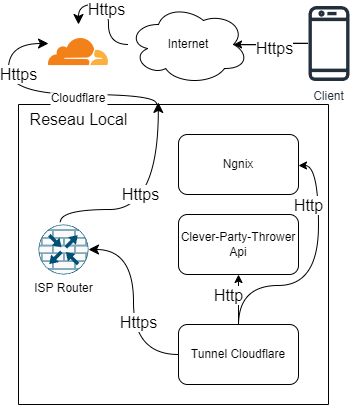
\includegraphics[width=\textwidth]{./images/shemaReseauDocker.drawio}
        \caption{Schema reseau Logique avec Docker}
        \label{fig:schemaDocker}
    \end{subfigure}
    \hfill
    \begin{subfigure}[b]{0.45\textwidth}
        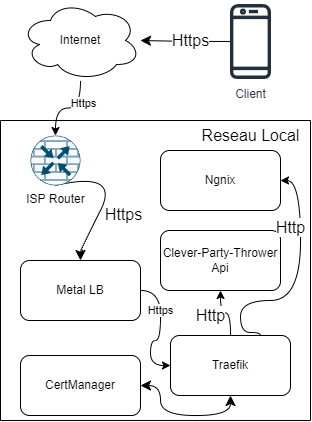
\includegraphics[width=\textwidth]{./images/shemaReseauKube.drawio}
        \caption{Schema reseau Logique avec Kubernetes}
        \label{fig:schemaKube}
    \end{subfigure}
    \caption{Le sens des differentes flèches représente le sens d'initialisation des connections}
    \label{fig:schemaReseau}
\end{figure}
    \newpage


    \section{Développement de l'application}\label{sec:developpement-de-l'application}
    \input{Développement de l'application}
    \newpage


    \section{Base de donnees}\label{sec:base-de-donnees}
    \subsection{Introduction}\label{subsec:introduction_base_de_donnee}
Dans le contexte de mon application \("\)Clever Party Thrower\("\), une base de données est nécessaire pour gérer diverses informations générées par les utilisateurs,
ainsi que pour stocker d'autres données essentielles au bon fonctionnement de l'application.
Cette section fournit un aperçu détaillé de la conception, du choix, des opérations et de la structure de la base de données.

\subsection{Choix de la base de données}\label{subsec:choix-de-la-base-de-donnee}
Le choix du système de base de données est un aspect crucial de tout projet, car il influence directement les performances et la fonctionnalité de l'application.
Comme je l'ai précisé dans la section d'analyse, j'ai choisi un système de base de données de type SQL, plus précisément PostgreSQL, pour ce projet.
La haute disponibilité offerte par PostgreSQL, grâce à ses fonctionnalités avancées de réplication de données, a été l'une des principales motivations de ce choix.

De plus, PostgreSQL offre une grande extensibilité.
Son système d'extensions permet d'ajouter facilement des fonctionnalités à la base de données.
Par exemple, l'extension PostGIS, qui facilite le stockage et la manipulation des données géographiques, a été particulièrement utile pour mon application,
en particulier pour la fonction de covoiturage qui nécessite le calcul de la distance entre deux points géographiques.

En outre, le caractère open source de PostgreSQL, sa réputation solide et ses performances de haut niveau en font un choix idéal pour mon projet.
Sa compatibilité avec de nombreux langages de programmation et ORMs, dont TypeOrm que j'ai utilisé pour le développement de l'application, a consolidé ce choix.

\subsection{Opérations sur la base de données}\label{subsec:operation-sur-la-base-de-donnees}
Les opérations sur la base de données sont principalement de nature CRUD (Create, Read, Update, Delete).
Cependant, avec l'introduction du système de covoiturage, des opérations plus complexes sont devenues nécessaires.
Par exemple, le calcul des distances entre différents points géographiques est une opération essentielle pour la coordination du covoiturage.

\subsection{Structure de données}\label{subsec:structure-de-donnees}
La structure de la base de données est illustrée dans la figure ci-dessous.
Cette structure a été conçue pour garantir une exécution efficace des opérations de la base de données, tout en assurant la cohérence et l'intégrité des données.
Elle comporte plusieurs tables, dont chaque instance contient des informations pertinentes et est liée à d'autres tables pour créer des relations significatives entre les différentes données.
Voici une brève description ce chaque table de la basse de donnees
\begin{itemize}
    \item address : Contient des informations sur les adresses.
    Chaque instance d'adresse est liée à une instance de \("\) country \("\) (via \("\) countryId \("\)) et à une instance de \("\) user\_entity\("\) (via \("\)ownerId\("\)).
    \item car : Contient des informations sur les voitures.
    Chaque instance de voiture est liée à une instance de \("\)user\_entity\("\) (via \("\)ownerId\("\)).
    \item carpool : Contient des informations sur le covoiturage.
    \item Chaque instance de covoiturage est liée à une instance de \("\)address\("\) (via \("\)startPointId\("\) et \("\)endPointId\("\)), une instance de \("\)car\("\) (via \("\)carId\("\)),
    une instance de \("\)event\("\) (via \("\)eventId\("\)), et une instance de \("\)user\_entity\("\) (via \("\)driverId\("\)).
    \item country : Contient des informations sur les pays.
    Il est lié à \("\) address\("\) (via \("\)id\("\)).
    \item  dates\_t\_user : Contient des informations sur les dates liées aux utilisateurs.
    Chaque instance est liée à une instance de \("\)event\_date\("\) (via \("\) eventDateId\("\)) et à une instance de \("\)event\_to\_user\("\) (via \("\) eventToUserId\("\)).
    \item dept : Contient des informations sur les dettes.
    Chaque instance est liée à une instance de \("\)event\("\) (via \("\) eventId\("\)), et à deux instances de \("\) user\_entity \("\) (via \("\) creditorId\("\) et \("\)debtorId\("\)).
    \item event : Contient des informations sur les événements.
    Chaque instance est liée à une instance de \("\)address\("\) (via \("\)addressId\("\)) .
    \item event_date : Contient des informations sur les dates d'événement.
    Chaque instance est liée à une instance de \("\)event\("\) (via \("\)eventId\("\)).
    \item event_to_user : Contient des informations sur la relation entre les événements et les utilisateurs.
    Chaque instance est liée à une instance de \("\)address\("\) (via \("\)addressString\("\)), une instance de \("\)event\("\) (via \("\)eventId\("\)), et une instance de \("\)user\_entity\("\) (via \("\)userId\("\)).
    \item route_entity : Contient des informations sur les itinéraires.
    Chaque instance est liée à deux instances de \("\)address\("\) (via \("\)startingId\("\) et \("\)destinationId\("\)), une instance de \("\)carpool\("\) (via \("\)carpoolId\("\)), et une instance de \("\)user\_entity\("\) (via \("\)pickupId\("\)) .
    \item shopping_list_item : Contient des informations sur les articles de la liste de courses.
    Chaque instance est liée à une instance de \("\)event\("\) (via \("\) eventId\("\)) et à une instance de \("\)user\_entity\("\) (via \("\)assignedId\("\)).
    \item spending : Contient des informations sur les dépenses.
    Chaque instance est liée à une instance de \("\)event\("\) (via \("\)eventId\("\)), une instance de \("\)shopping\_list\_item\("\) (via \("\)shoppingListItemId\("\)), et une instance de \("\)user\_entity\("\) (via \("\)buyerId\("\)).
    \item user_entity : Contient des informations sur les utilisateurs.
    Chaque instance est liée à une instance de \("\)address\("\) (via \("\)addressId\("\)).
\end{itemize}

Le schema est disponible \ref{fig:dbSchema}ici


    \section{Historique du projet}\label{sec:historique-du-projet}
    \subsection{Introduction}\label{subsec:introduction2}
Dans cette section, nous examinerons l'évolution du projet, depuis sa phase de conceptualisation jusqu'à sa réalisation finale, en soulignant les différentes difficultés rencontrées en cours de route.
Nous mettrons également en lumière les jalons clés du projet, les ajustements de la planification et les interactions avec le rapporteur.

\subsection{Chronologie du projet}\label{subsec:chronologie-du-projet}
Le projet a officiellement débuté en septembre 2022, marqué par une première phase d'échanges intenses avec de potentiels utilisateurs et de définition des objectifs.
Des étapes clés ont jalonné notre progression, telles que la finalisation du cahier des charges et la sélection des technologies en octobre 2022,
le commencement du développement dans la même période, et enfin, le déploiement de la premiere version l'application en juin 2023.

\subsection{Réunions et interactions avec le client/rapporteur}\label{subsec:reunions-et-interactions-avec-le-client/rapporteur}
Au cours du projet, j'ai eu plusieurs réunions avec mon rapporteur.
Ces réunions ont été l'occasion de discuter de l'avancement du projet, de recueillir des retours constructifs et d'adapter notre approche en conséquence.
Par exemple, lors de la réunion de validation du sujet en octobre, nous avons convenu que la conception de l'application
devrait être suffisamment flexible pour permettre l'ajout de nouvelles fonctionnalités à l'avenir, comme un système de covoiturage.

\subsection{Évolution des choix techniques et stratégiques}\label{subsec:evolution-des-choix-techniques-et-strategiques}
Au fil du projet, certaines modifications ont été nécessaires.
Ces ajustements étaient principalement dus à RxJS. Initialement, j'avais prévu de concevoir le projet de manière à ce que l'application soit réactive sur l'ensemble du stack.
Cependant, après une discussion éclairante avec mon rapporteur, M. Noel,
nous avons décidé de construire le projet de manière classique tout en envisageant l'ajout de la réactivité dans une phase future.

\subsection{Defits lors du developement}\label{subsec:defits-lors-du-developement}
Lors du develepement du projets plusieurs defit on du etre surmonter

\subsubsection{L'algorithme des dettes}
Le développement d'un algorithme capable de répartir les différents coûts d'un événement entre les utilisateurs s'est avéré être un défi.
Non seulement il fallait que les différentes dépenses existantes à un instant T soient réparties entre les différents participants, mais il fallait aussi permettre aux participants de continuer à ajouter des dépenses, même une fois qu'un utilisateur a remboursé ses dettes.

Au départ, l'algorithme était plutôt simple : récupérer toutes les dépenses pour un événement donné dans la base de données, calculer le total des dépenses pour l'événement et créer une dette par participant, dont la valeur est le total divisé par le nombre de participants.

Cependant, cet algorithme n'était pas satisfaisant pour plusieurs raisons, principalement le manque de possibilité de spécifier à qui les dettes doivent être remboursées.
J'ai donc décidé de changer d'approche.
Au lieu de calculer le total des dépenses pour un événement, nous allons calculer la balance totale de chaque participant.

Pour cela, lors du calcul des dettes, on crée une carte associant un participant à une balance.
Une fois que la balance de chaque participant est créée sur la base de toutes les dépenses, on parcourt cette carte afin de créer des paires de participants.
L'objectif est de trouver le participant avec la balance la plus positive et celui avec la balance la plus négative.
Une fois que l'on a cette paire, on peut créer une dette entre ces deux utilisateurs de sorte à ce que l'un ou les deux voient leur balance revenir à zéro.
Après avoir créé cette dette, on met à jour la balance des deux utilisateurs.
On continue ainsi jusqu'à ce que toutes les balances des utilisateurs valent zéro

À première vue, cette stratégie fonctionne.
Cependant, comme je l'ai découvert plus tard dans le développement, elle présente plusieurs problèmes majeurs.
Premièrement, cet algorithme ne permet pas aux utilisateurs de marquer une dette comme remboursée et que cela persiste au travers des différents calculs.
Deuxièmement, les participants ne peuvent pas créer de dépenses entre eux et donc un participant qui aurait par exemple participé à un covoiturage ne paierait pas plus qu'un participant qui se serait déplacé par ses propres moyens.
Troisièmement, une dépense est obligatoirement répartie entre tous les participants.

Pour remédier à ces problèmes, il a fallu modifier les dépenses afin de permettre de sélectionner un acheteur et un bénéficiaire.
Désormais, chaque achat dans la liste des courses, par exemple, crée une dépense entre l'acheteur et chacun des bénéficiaires.
Un champ permettant de conserver la balance d'un utilisateur a été ajouté à l'entité EventToUser afin d'optimiser les calculs (plus besoin de parcourir toutes les dépenses pour pouvoir générer les dettes).
Pour gérer le remboursement des dettes, nous profitons de l'ajout d'un acheteur à une dépense.
Lorsqu'un participant marque une dette comme remboursée, une dépense de valeur opposée est créée entre le créancier et le débiteur afin de contrebalancer la dette.
Cette dernière est alors supprimée.

La solution mise en place permet de gérer efficacement le remboursement des dettes et de répartir les dépenses parmi les consommateurs,
optimisant ainsi les calculs de remboursement.
Grâce à une modification récente, les participants peuvent désormais diviser une dépense de manière inégale ou choisir de ne pas la répartir entre tous les participants,
ajoutant une couche supplémentaire de flexibilité à cet algorithme.

\subsubsection{le cluster kubernetees}
La conception et la mise en place d'un cluster Kubernetes ont probablement été les défis majeurs de ce projet.
L'apprentissage des différents outils, la conception du cluster et son déploiement ont été des étapes cruciales.
Au début du projet, j'étais totalement novice avec Kubernetes et Ansible n'était pour moi qu'un nom.

J'ai donc dû m'initier au fonctionnement de Kubernetes et aux différents outils pouvant être utilisés en parallèle.
Mes recherches m'ont conduit à découvrir une immense communauté de passionnés qui ont appris à utiliser Kubernetes
et ont créé de la documentation à ce sujet pour le plaisir ou pour des fins professionnelles.
Techno Tim, l'un d'entre eux, a créé une série de vidéos où il partage les différentes configurations mises en place
dans son micro datacenter qu'il gère chez lui.
C'est en découvrant ces vidéos que j'ai commencé à apprendre comment configurer Kubernetes et utiliser Ansible.

Grâce à ces nouvelles connaissances, j'ai décidé de mettre en place sur l'un de mes serveurs un cluster qui,
grâce à la virtualisation, serait hautement disponible.
En réalité, seule la redondance du cluster Kubernetes est intégrée ;
il n'y a pas de redondance au niveau matériel car je n'avais pas les moyens de l'implémenter.

J'ai donc commencé par créer des machines virtuelles (VM) sur mon hyperviseur (Proxmox).
Après une mauvaise manipulation, j'ai décidé de recommencer depuis le début.
Je me suis alors rendu compte que créer les VM manuellement n'était pas l'idéal,
mais je ne voulais pas mettre en place un système de MaaS (Metal as a Service) qui aurait trop sollicité mon serveur.
J'ai donc choisi une solution intermédiaire : je n'ai pas complètement automatisé la configuration et le provisionnement
de machines virtuelles, mais j'ai cherché à simplifier considérablement le processus.

C'est alors que j'ai découvert deux outils formidables : les templates de VM qemu et CloudInit.
Grâce à ces outils, je pouvais facilement créer des machines virtuelles avec mes paramètres,
et modifier ceux-ci via CloudInit avant même de démarrer la machine virtuelle.

Fort de cette nouvelle découverte, j'ai mis en place sept VM dédiées au cluster Kubernetes :
trois serviront de plans de contrôle et quatre de nœuds d'exécution.

Le projet nécessitant une infrastructure d'hébergement et étant conteneurisé, tout s'alignait parfaitement.

Après des jours d'expérimentation manuelle avec Kubernetes via kubectl, Lens et Portainer, j'ai décidé de ne plus vouloir
d'un cluster unique et fragile comme un flocon de neige.
Je me suis tourné vers Ansible, un outil dont j'avais entendu beaucoup de bien, afin de définir mon infrastructure en tant que code.

J'ai cherché comment configurer un cluster Kubernetes via Ansible et j'ai découvert l'existence d'une communauté de passionnés
qui ont créé et publié en open-source des playbooks Ansible complets permettant de mettre en place un cluster.

Dans cette communauté, j'ai retrouvé Techno Tim qui a, lui aussi, contribué en adaptant un playbook existant
afin de déployer un cluster hautement disponible.
J'ai donc décidé de partir de son projet pour construire mon infrastructure.
J'ai ajouté au script original cert-manager, Traefik, Rancher, Longhorn et ArgoCD\@.

L'ajout de cert-manager et Traefik a été plutôt simple, mais l'intégration de Rancher s'est avérée plus complexe pour plusieurs raisons.

Premièrement, mon serveur était très limité en ressources pour ce type de tâche, encore plus à cause de la virtualisation
et du niveau de redondance nécessaire à la haute disponibilité.
Deuxièmement, la version de Rancher que j'essayais d'installer à ce moment-là n'était tout simplement pas compatible avec K3S
(l'implémentation de Kubernetes que j'avais décidé de déployer).
Enfin, après avoir changé de version de Rancher et sélectionné une version compatible avec K3S,
je me suis rendu compte que cette version n'était pas compatible avec la version spécifique de K3S que j'avais choisie.
J'ai donc dû changer une fois de plus de version de Rancher.
J'ai finalement pu finaliser la mise en place de mon cluster.

Deux mois plus tard, j'ai voulu apporter une modification au cluster, plutôt simple : j'ai voulu ajouter un certificat TLS.
Au lieu de simplement modifier le cluster existant, j'ai décidé de tirer profit de mon IaC pour pérenniser ce changement.
J'ai donc modifié les détails dans le playbook et je l'ai lancé.
Malheureusement, le cluster ne répondait plus\ldots

En fait, en raison d'un manque chronique de ressources, certains processus essentiels
à Kubernetes n'avaient pas pu être exécutés à temps, ce qui a entraîné l'arrêt de son fonctionnement.
J'ai donc décidé de recréer le cluster à partir de zéro.
Cependant, mon playbook, qui deux mois plus tôt fonctionnait parfaitement, ne fonctionnait plus du tout.

Après de longues heures de débogage, je n'arrivais pas à trouver la cause du problème,
même après être revenu à la dernière version du playbook qui avait servi à déployer le cluster.
Impossible de redéployer le cluster.
Rien n'avait changé dans le reste de l'infrastructure pourtant.

Le playbook affichait toujours la même erreur : "helm: jetstack repository not found". %todo: change error message for the real one
Le problème est que la commande d'ajout de ce référentiel est bien exécutée et sans erreurs et que lorsque je teste manuellement,
le référentiel est bien ajouté à Helm et disponible.

J'ai consacré de nombreuses heures à essayer de résoudre ce problème, mais sans succès.
C'était frustrant et déroutant, car je n'avais apporté aucun changement majeur au playbook depuis son dernier déploiement réussi.

Face à ce blocage, j'ai été contraint de reconsidérer l'approche technique pour le déploiement de mon projet.
J'ai donc décidé de mettre Kubernetes de côté et de me concentrer sur Docker-compose.
Bien que ce ne soit pas la solution initiale envisagée,
Docker-compose m'a permis de poursuivre le développement du projet tout en conservant l'aspect conteneurisé de l'application.

\paragraph{Le choix de Docker-compose}


Docker-compose s'est révélé être une alternative efficace à Kubernetes, grâce à sa simplicité d'utilisation et à sa moindre consommation de ressources.
Il m'a permis de définir et de gérer plusieurs conteneurs comme un ensemble de services interconnectés, ce qui correspondait parfaitement aux besoins de mon projet.
De plus, la préparation d'un fichier docker-compose était prévue dans le cadre du projet pour accompagner les clients
potentiels qui ne seraient pas en mesure de déployer le projet sur Kubernetes mais qui pourraient aisément l'exploiter via Docker-compose.

La migration vers Docker-compose s'est faite sans difficultés majeures, étant donné ma familiarité avec Docker et le fait que mon application était déjà conteneurisée.
Quelques ajustements dans le fichier docker-compose.yml ont été suffisants pour rendre mon application pleinement opérationnelle.

Ce revirement de situation m'a libéré du temps pour me concentrer sur d'autres aspects du projet,
tels que le développement de nouvelles fonctionnalités et l'amélioration de l'expérience utilisateur.
Malgré une certaine déception de ne pas avoir pu implémenter Kubernetes comme initialement prévu, je reste satisfait du résultat final.
Docker-compose a parfaitement répondu à mes besoins et m'a permis de mener à bien mon projet.

Pour conclure, bien que la tentative d'implémentation de Kubernetes ait été un défi majeur qui n'a pas abouti comme je l'espérais,
ce projet reste une riche expérience d'apprentissage.
J'ai pu approfondir ma compréhension des outils de déploiement et d'orchestration de conteneurs et développer des compétences précieuses en matière de débogage et de résolution de problèmes.
Malgré les difficultés rencontrées, je suis fier du travail accompli et je reste déterminé à explorer davantage Kubernetes dans le cadre de futurs projets.

\subsubsection{le client graphql}



%
%    Historique du projet
%    Planning de réalisation et respect de celui-ci
%    Bilan des rencontres avec le client et/ou le rapporteur
%    Évolution des choix dans le temps
%
%    Versioning
%    Utilisation de GitHub
%    Commits réguliers tout au long du projet
%
%    Produit fini et démonstration
%    Testabilité du code/produit
%    Procédure d'installation
%    Présentation de la réalisation (validation par le client, déploiement en production)
%
%    Bilan
%    Analyse critique du projet (points forts, points faibles)
%    Améliorations envisageables
%    Plan pour le futur
%    ce que j'aurais fait autrement
%
%    Ressources utilisées
%    Sources de ressources intellectuelles ou d'exploitation (bibliographie, licences logicielles, etc.)
%
%    Conclusion
%    Récapitulatif des objectifs atteints
%    Importance et implications du projet


    %\backendx
    % La db (shema+ ORM + GDPR)
    % graphql
    % NestJs

    % Le front end
    % agular
    % apollo
    % les service
    % l'authentification par token


%    \section{hebergement}
    % proxmox
    % ansible
    % kubernetes
    % traefik, certmanager & https
    % longhorn & rancher
    % reseau (ce qui aurais du etre fait et ce qui est fait)
%   docekr-compose
    \newpage
\end{document}
